\chapter{Sound and Audio}

Sound is a physical phenomenon caused by vibration of material, such as a sarangi string (\textnp{\footnotesize{सारङ्गीकाे तार}}) or a madal (\textnp{\footnotesize{मादल}}). This type of vibration triggers pressure wave fluctuations in the air around the material. The pressure waves propagate through the air in a wave-like motion. When a wave reaches the human ear, We hear a sound.




\section{Sound, Representation and Formats}
\subsection{Basic Sound Concept}
Sound is produced by the vibration of matter. During the vibration, pressure variations are created in the air surrounding it. The pattern of this oscillation (see Figure \ref{fig:oscillation}) is called \textit{waveform}. 


%@@@@@@@@@@@@@@@@@@@@@@@@@@@@@@@@@@@@
%									@
%			FIGURE					@
%									@
%@@@@@@@@@@@@@@@@@@@@@@@@@@@@@@@@@@@@

\begin{figure}[ht!]
	\centering
	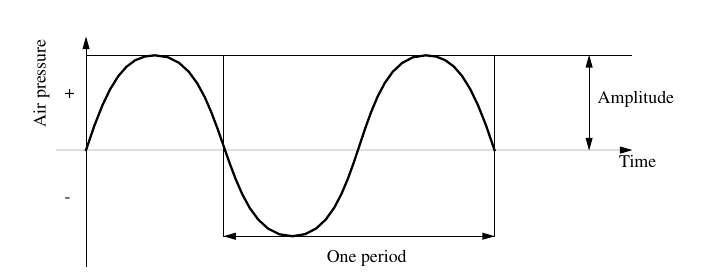
\includegraphics[width=\textwidth]{pressure-wave-osc}
	\caption{Pressure wave oscillation in the air.}{\label{fig:oscillation}}
\end{figure}


This wave form occurs repeatedly at regular \textit{intervals} or \textit{periods}. Sound waves have a natural origin, so they are never absolutely uniform or periodic. 
\begin{itemize}
	\item A sound that has a recognizable periodicity is referred to as \textit{music}.
	\item Examples of \textit{periodic} sound: sounds generated by musical
	instruments, vocal sounds, wind sounds, or a bird’s twitter.
	\item Examples of \textit{non-periodic} sounds: drums, coughing, sneezing, etc.
\end{itemize}

\subsubsection{Frequency}
A sound's frequency is the \textit{reciprocal value of its period}. The frequency represents the number of periods per second and is measured in \gls{hz} or \gls{cps}.

A common abbreviation is \gls{khz}, which describes 1,000 oscillations per second, corresponding to 1,000Hz. Sound processes that occur in liquids, gases, and solids are classified by frequency range:

\begin{multicols}{2}
\begin{itemize}
	\item Infrasonic: 0 to 20\gls{hz}
	\item Audiosonic: 20\gls{hz} to 20\gls{khz}
	\item Ultrasonic: 20\gls{khz} to 1GHz
	\item Hypersonic: 1GHz to 10THz
\end{itemize}
\end{multicols}


 Multimedia systems make use of sound only within frequency range of human hearing. Sound within human hearing range is called \textit{audio}. The waves in the audiosonic frequency range are called \textit{acoustic signals}. 

\begin{itemize}
	\item Speech is an acoustic signal produced by humans.
	\item Music signals have a frequency range between 20\gls{hz} and 20\gls{khz}.
	\item Beside speech and music, we denote any other audio signal as \textit{noise}.
\end{itemize}


\subsubsection{Amplitude}
A sound has a property called \textit{amplitude}, which humans perceive subjectively as
loudness or volume. The amplitude of a sound is a measuring unit used to deviate the
pressure wave from its mean value (idle state).

\subsection[Representation]{Sound Representation}
The smooth, continuous curve of a sound waveform is not directly represented in
a computer. A computer measures amplitude of the waveform at regular time
intervals to produce a series of numbers. Each of these measurements is a \textit{sample}. Figure {\ref{fig:wave-sampling}} shows one period of a digitally sampled wave.

%@@@@@@@@@@@@@@@@@@@@@@@@@@@@@@@@@@@@
%									@
%			FIGURE					@
%									@
%@@@@@@@@@@@@@@@@@@@@@@@@@@@@@@@@@@@@

\begin{figure}[H]
	\centering
		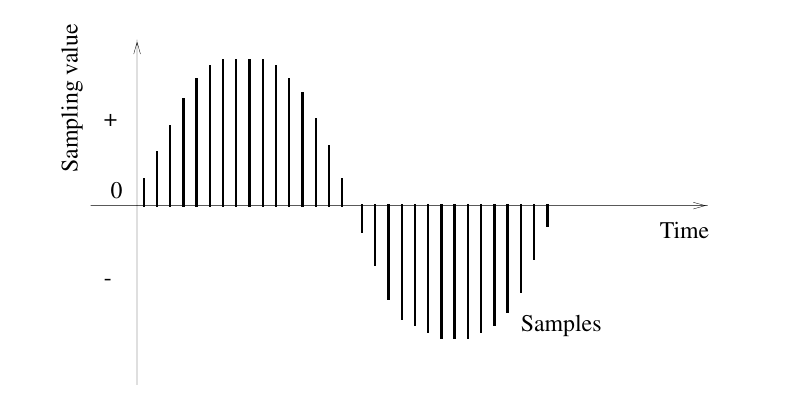
\includegraphics[width=0.8\textwidth]{sampling-a-wave}
	\caption{Sampling a wave.}{\label{fig:wave-sampling}}
\end{figure}


The mechanism that converts an audio signal into a sequence of digital samples is called an \gls{adc} and a \gls{dac} is used to achieve the opposite conversion.

\subsection{Sampling Rate}
The rate at which a continuous wave form is sampled (see Figure {\ref{fig:wave-sampling}}) is called the \textit{sampling rate}. It is measured in \gls{hz}. 

For example, CDs are sampled at a rate of \(44,100\)\gls{hz}, which may appear to be above the frequency range perceived by humans. However, the bandwidth in this case, \(20,000Hz-20Hz = 19,980Hz\) that can represent a digitally sampled audio signal is only about half as big as a CD's sampling rate, because CDs use the \textbf{Nyquist sampling theorem}\footnote{Nyquist’s Sampling Theorem: The Sampling frequency for a signal must be at least twice
	the highest frequency component in the signal}. This means
that a sampling rate of $ 44,100Hz $ covers only frequencies in the range from $ 0Hz $ to
$ 22,050Hz $. This limit is very close to the human hearing capability.


\subsection{Quantization}
The digitization process requires two steps. 
\begin{itemize}
	\item First the analog signal must be sampled. This means that only a discrete set of values is retained at (generally regular) time
	or space intervals. 
	
	\item The second step involves quantization. The \textit{quantization} process consists of converting a sampled signal into a signal that can take only a limited number of values.
\end{itemize}
 
An 8-bit quantization provides 256 possible values, while a 16-bit quantization in \gls{cd} quality results in more than $ 65,536 $ possible values. Figure \ref{fig:3bit-quantization} shows a 3-bit quantization.

%%%%%%%%%%%%%%%%%%%%%%%%%%%%%%%%%%%%%%%%%
%										%
%				FIGURE				   	%
%										%
%%%%%%%%%%%%%%%%%%%%%%%%%%%%%%%%%%%%%%%%%
\begin{figure}[H]
	\centering
		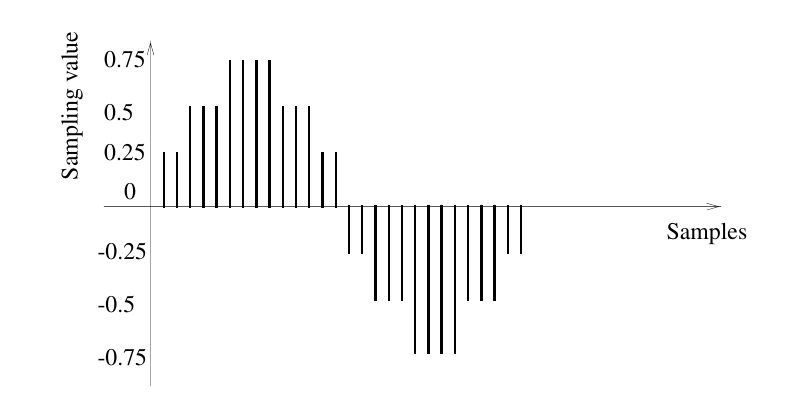
\includegraphics[width=\textwidth]{3-bit-quantization}
	\caption{3-bit quantization.}{\label{fig:3bit-quantization}}
\end{figure}

%-------------------FIGURE END---------------------------

The values transformed by a 3-bit quantization process can accept eight different
characteristics: \(0.75, 0.5, 0.25, -0.25, -0.5, -0.75, and\, -1\), so that we obtain an
“angular-shape” wave. This means that the lower the quantization (in bits), the more the
resulting sound quality deteriorates.

\subsection{Sound Hardware}
Before sound can be processed, a computer needs input/output devices. Microphone
jacks and built-in speakers are devices connected to an \gls{adc} and \gls{dac}, respectively for the input and output of audio.

\subsection{Formats}
\begin{itemize}
	\item Popular audio file formats include:
		\begin{itemize}
			\item \texttt{.au}(Origin: Unix, Sun),
			\item \texttt{.aiff}(Mac),
			\item \texttt{.wav} (PC)
		\end{itemize}
	\item Compression can be utilized in some of the above but is not Mandatory.
	\item A simple and widely used (by above) audio compression method is \gls{adpcm}.
			\begin{itemize}
				\item Based on past samples, it predicts the next sample and
				encodes the difference between the actual value and the
				predicted value.
			\end{itemize}
		\item Many formats linked to audio applications.
		\item Most audio formats use compression.
\end{itemize}

Audio format defines the quality and loss of audio data. Based on application different type of audio format are used. Audio formats are broadly divided into three parts:

\begin{enumerate}
	\item \textit{Uncompressed Format}. Example: \gls{wav}, \gls{aiff}, AU.
	\item \textit{Lossy Compressed format}. Example: \gls{mp3}, \gls{aac}, \gls{wma} Lossy.
	\item \textit{Lossless Compressed Format}. Example: \gls{flac}, \gls{alac}.
\end{enumerate}

 
\section[Basic Music (MIDI)]{Basic Music (MIDI)}
Music can be described in a symbolic way. On paper, we have the full scores.
Computers and electronic musical instruments use a similar technique, and most of
them employ the Musical Instrument Digital Interface (MIDI), a standard developed in
the early 1980s. The \gls{midi} standard defines how to code all the elements of musical
scores, such as sequences of notes, timing conditions, and the instrument to play each
note.

The \gls{midi} interface between electronic musical instruments and computers is a small piece of equipment that plugs directly into the computer's serial port and allows transmission of music signals. 

\subsection[Concepts]{MIDI Concepts}
MIDI represents a set of specifications used in instrument development so that
instruments from different manufacturers can easily exchange musical information. A MIDI interface is composed of two different components:

\begin{itemize}
	\item \textbf{Hardware} to connect the equipment. \gls{midi} hardware specifies the physical connection of musical instruments. It adds a \gls{midi} port to an instrument, it specifies a \gls{midi} cable (that connects two instruments), and processes electrical signals received over the cable.
	
	\item \textbf{A data format} that encodes information to be processed by the hardware. The MIDI data format does not include the encoding of individual sampling values, such as audio data formats. Instead, \gls{midi} uses a specific data format for each instrument, describing things like the start and end of scores, the basis frequency, and loudness, in addition to the instrument itself.
	
\end{itemize}
The MIDI data format is digital and data are grouped into \gls{midi} messages. When
a musician plays a key, the \gls{midi} interface generates a \gls{midi} message that defines the start of each score and its intensity. This message is transmitted to machines connected to the system. As soon as the musician releases the key, another signal (\gls{midi} message) is created and transmitted.

\subsection[Components]{Components of a MIDI System}

\subsubsection*{Synthesizer}
	\begin{itemize}
	\item It is a sound generator (various pitch, loudness, tone colour).
	\item A good (musician's) synthesizer often has a microprocessor, keyboard, control panels, memory, etc. 
\end{itemize}

\subsubsection*{Sequencer}
	\begin{itemize}
		\item It can be a standalone unit or a software program for a personal computer.
		\item It has one or more MIDI INs and MIDI OUTs. 
	\end{itemize}

\subsubsection*{Track}	
	\begin{itemize}
		\item Track in sequencer is used to organize the recordings.
		\item Tracks can be turned on or off on recording or playing back. 
	\end{itemize}
	
\subsubsection*{Channel}
	\begin{itemize}
		\item MIDI channels are used to separate information in a MIDI system.
		\item There are 16 MIDI channels in one cable.
		\item Channel numbers are coded into each MIDI message. 
	\end{itemize}
	
\subsubsection*{Timbre}
	\begin{itemize}
		\item The quality of the sound, e.g., flute sound, cello sound, etc.
		\item Multitimbral - capable of playing many different sounds at the same time (e.\ g.\ , piano, brass, drums, etc).
	\end{itemize}
	
\subsubsection*{Pitch}
	\begin{itemize}
		\item Musical note that the instrument plays. 
	\end{itemize}
		
\subsubsection*{Voice}
	\begin{itemize}
		\item Voice is the portion of the synthesizer that produces sound.
		\item Synthesizers can have many (12, 20, 24, 36, etc.) voices.
		\item Each voice works independently and simultaneously to produce sounds of different timbre and pitch.
	\end{itemize}
		
\subsubsection*{Patch}
	\begin{itemize}
		\item The control settings that define a particular Timbre.
	\end{itemize}



\subsection[Devices]{MIDI Devices}
%Through the MIDI interface, a computer can control output of individual instruments. On the other hand, the computer can receive, store or process coded musical data through the same interface. The data are generated with a \textit{keyboard} and reproduced through a sound generator. A \textit{sequencer} can store data. Further, it may
%also modify the musical data. In a multimedia system, the sequencer is a computer
%application.

%An instrument that complies with both components defined by the MIDI standard
%is a MIDI device (e.g., a synthesizer) able to communicate with other MIDI devices
%over channels. The MIDI standard specifies 16 channels. A MIDI device is mapped
%onto a channel. Musical data transmitted over a channel are reproduced in the synthe-
%sizer at the receiver’s end. The MIDI standard identifies 128 instruments by means of numbers, including noise effects (e.g., a phone ringing or an airplane take-off). For
%example:
%\begin{itemize}
%	\item  $ 0 $ specifies a piano
%	\item $ 12 $ a marimba
%	\item $ 40 $ a violin, and 
%	\item $ 73 $ a flute
%\end{itemize}
%
%Some instruments enable a user to play one single score (e.g., a flute) exclusively,
%while other instruments allow concurrent playing of scores (e.g., an organ). The maximum number of scores that can be played concurrently is an important property of synthesizers. This number can vary between 3 and 16 scores per channel.

A computer uses the \gls{midi} interface to control instruments for playout. The computer can use the same interface to receive, store, and process encoded musical data. 

\begin{itemize}
	\item In the \gls{midi} environment, these data are generated on a \textit{keyboard} and played out by a \textit{synthesizer}.
	\item A typical synthesizer is similar to a regular piano keyboard.
	\item A \textit{sequencer} is used to buffer or modify these data. In a multimedia application, the sequencer is a computer application.
\end{itemize}

The heart of any \gls{midi} system is the \gls{midi} \textit{synthesizer} device. A typical synthesizer looks like a simple piano keyboard with a panel full of buttons. Most synthesizers have the following common components:

\subsubsection*{Sound Generator}
\begin{itemize}
	\item The principal purpose of the generator is to produce an audio signal that
	becomes sound when fed into a loudspeaker. 
	
	\item By varying the voltage oscillation of the audio signal, a sound generator changes the quality of the sound – its pitch, loudness and tone – to create wide variety of
	sounds and notes.
\end{itemize}

\subsubsection*{Microprocessor}
\begin{itemize}
	\item The microprocessor communicates with the keyboard to know what notes the musician is playing, and with the control panel to know what
	commands the musician wants to send to the microprocessor. 
	\item The microprocessor then specifies note and sound commands to the sound generators.
\end{itemize}


\subsubsection*{Keyboard}
\begin{itemize}
	\item The keyboard affords the musician's direct control of the synthesizer.
	\item Pressing keys on the keyboard signals the microprocessor knows what
	notes to play and how long to play them.
\end{itemize}


\subsubsection*{Control Panel}
\begin{itemize}
	\item The control panel controls those functions that are not directly
	concerned with notes and durations. 
	\item It includes: 
		\subitem a \textit{slider} that sets the overall volume of the synthesizer, 
		\subitem a \textit{button} that turns the synthesizer on and off, and 
	\subitem a \textit{menu} that calls up different patches for the sound
	generators to play.
\end{itemize}


\subsubsection*{Auxiliary Controller}
They are available to give more control over the notes played on the
keyboard.

\subsubsection*{Memory}
Synthesizer memory is used to store patches for the sound generators
and settings on the control panel.\\

\noindent There are many other \gls{midi} devices that augment the standard synthesizer in a \gls{midi} system. Examples are drum machines which specialize in percussion sound's and rhythms, the master keyboard which increases the quality of the synthesizer keyboard, guitar controllers, guitar synthesizers, drum pad controllers and so on.

\subsection[Messages]{MIDI Messages}
 \gls{midi} messages are used by \gls{midi} devices to communicate with each other.
 
% \subsubsection[Structure]{Structure of MIDI Messages} 
 \subsubsection*{Structure of MIDI Messages} 

 \begin{itemize}
 	\item \gls{midi} message includes a \textit{status byte} and up to two \textit{data bytes}.
 	\item \textit{Status byte}
 	\begin{itemize}
 		\item The most significant bit of status byte is set to 1.
 		\item The 4 low-order bits identify which channel it belongs to.
 		\item The 3 remaining bits identify the message.
 	\end{itemize}
 	\item The most significant bit of data byte is set to 0. 
 \end{itemize}

%\subsubsection[Classification]{Classification of MIDI Messages}
\subsubsection*{Classification of MIDI Messages}

%@@@@@@@@@@@@@@@@@@@@@@@@@@@@@@@@@@@@
%									@
%			FIGURE					@
%									@
%@@@@@@@@@@@@@@@@@@@@@@@@@@@@@@@@@@@@
\begin{figure}[ht!]
	\centering
	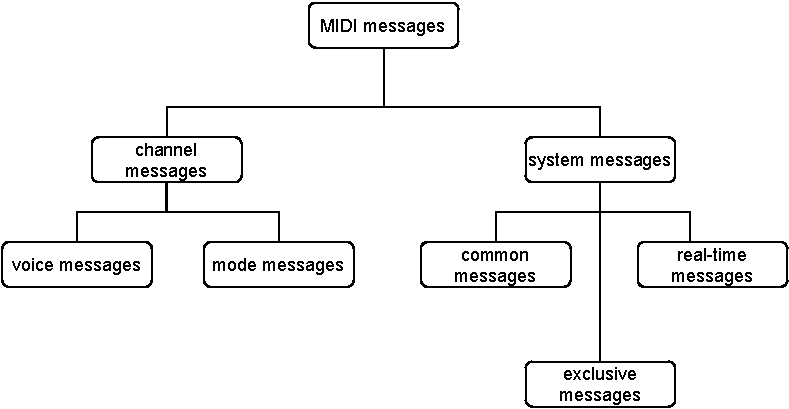
\includegraphics[width=0.9\textwidth]{midi-messages}
	\caption{Classification of \gls{midi} messages.}\label{fig:midi-messages}
\end{figure}

\begin{enumerate}[label=\Alph*)]
	\item \textbf{Channel messages}:  Messages that are transmitted on individual channels rather than globally to all devices in the \gls{midi} network.
	
		\begin{enumerate}[label=\alph*)]
			\item \textbf{Channel voice messages}
			
			    \begin{itemize}
			    	\item Instruct the receiving instrument to assign particular sounds to its voice.
			    	\item Turn notes on and off.
			    	\item Alter the sound of the currently active note or notes.
			    \end{itemize}
		    
		\item \textbf{Channel mode messages}
		
		\begin{itemize}
			\item Channel mode messages are a special case of the Control Change message. The difference between a Control message and a Channel Mode message is in the first data byte. 
			
			\item Channel mode messages determine how an instrument will process \gls{midi} voice messages. 
		\end{itemize}
		
		
		\end{enumerate}
	
	\item \textbf{System Messages}: System messages carry information that is not channel specific, such as timing signal for synchronization, positioning information in pre-recorded \gls{midi} sequences, and detailed setup information for the destination device.  
	  \begin{enumerate}
	  	\item \textbf{System real-time messages}: messages related to synchronization 
	  	\item \textbf{System common messages}: are commands that prepare sequencers and
	  	synthesizers to play a song. They are used for song selection, tuning the
	  	synthesizers etc.
	  	 \item \textbf{System exclusive message}: 
	  	 \begin{itemize}
	  	 	\item Messages related to things that cannot be standardized.
	  	 	\item Addition to the original \gls{midi} specification. 
	  	 	\item It is just a stream of bytes, all with their high bits set to 0, bracketed by a pair of system exclusive start and end messages.
	  	 \end{itemize}
	  \end{enumerate}
  
 
\end{enumerate}

\subsection[Standards]{MIDI Standards}
\begin{itemize}
	\item The \gls{midi} clock is used by a receiver to synchronize itself to the sender’s clock.
	\item To allow synchronization, 24 identifiers for each quarter note are transmitted. 
	\item Alternatively, the \gls{smpte} timing code
	can be sent to allow receiver-sender synchronization. 
	\item \gls{smpte} defines a frame format by
	\(hours:minutes:seconds:\), for example \(30\, frames/s\). This information is transmitted in a rate that would exceed the bandwidth of existing \gls{midi} connections.
	\item The \gls{midi} time code is normally used for synchronization because it does not transmit the entire time representation of each frame.
\end{itemize}


\subsection[Software]{MIDI Software}
Once a computer is connected to a \gls{midi} system, a variety of \gls{midi} applications can run on it. Digital computers afford the composer or sound designer unprecedented levels of control over the evolution and combination of sonic events.

The software applications generally fall into four major categories:

\subsubsection*{Music recording and performance applications}
This category of applications provide functions such as recording of \gls{midi} messages as they enter the computer from other \gls{midi} devices, and possibly editing and playing back the messages in performance.
			
 \subsubsection*{Musical notations and printing applications}
This category allows writing music using traditional musical notation. The user can then play back the music using a performance program or print the music on paper for live performance or publication.
			
\subsubsection*{Synthesizer patch editors and librarians}
These programs allow information storage of different synthesizer patches on the computer's memory and disk drives, and editing of patches on the computer.
			
\subsubsection*{Music education applications}
These software applications teach different aspects of music using the computer monitor, keyboard and other controllers of attached \gls{midi} instruments.		


\section{Speech}
\subsection{Concept}
Speech can be processed by humans or machines. The field of study of the handling of digitized speech is called digital speech processing.

Speech is based on spoken languages, which means that it has a semantic content. Human beings use their speech organs without the need to knowingly control the generation of sounds. Speech understanding means the efficient adaptation to speakers and their speaking habits. 

%Despite the large number of different dialects and emotional pronunciations, we can understand each other’s language. The
%brain is capable of achieving a very good separation between speech and interference,
%using the signals received by both ears. It is much more difficult for humans to filter signals received in one ear only. The brain corrects speech recognition errors because it
%understands the content, the grammar rules, and the phonetic and lexical word forms.

The human speech signal comprises a subjective lowest spectral component known as the \textit{pitch}, which is not proportional to frequency. The human ear is most sensitive in the range of $ 600 Hz $ to $ 6000 Hz $ Speech signals have two important characteristics that can be used by speech processing applications:

\begin{itemize}
	\item Voiced speech signals have an almost periodic	structure over a certain time interval, so that these signals remain \textit{quasi-stationary} for about $ 30ms $.
	
	\item The spectrum of some sounds have characteristic maxima that normally involve up to five frequencies. These frequency maxima, generated when speaking, are called \textit{formants}. By definition, a \textit{formant} is a characteristic component of the quality of an utterance.
\end{itemize}

%A machine can also support speech generation and recognition. With computers, one
%can synthetically generate speech, where the generated signals do not sound quite
%natural but can be easily understood. on the other hand, a
%voice can sound natura,l but may be very difrcult to understand. Speech recognition
%often uses matching rules or statistically based methods. Problems are caused when
%dialects, emotional pronunciation and environmental noises are part of the audio
%signal. There are, and will continue to be in the near future, considerable differences
%between the speech generation and recognition efficiencies/capabilities of the human
%brain and a high-performance computer.

\subsubsection*{Speech Synthesis}
Computers can translate an encoded description of a message into speech. This scheme is called \textit{speech synthesis}. A particular type of synthesis is text-to-speech conversion.

Speech recognition is normally achieved by drawing various comparisons. The problems in speech recognition affecting the recognition quality
include dialects, emotional pronunciations, and environmental noise. 

\subsection[Generation]{Speech Generation/Output}

A major challenge in speech output is how to generate these signals in real time for a speech output system to be able, for instance, to convert text to speech automatically. Some applications (e.\ g.\ , time announcements) handle this task with a limited vocabulary, but most use an extensive if not unlimited vocabulary.

The speech, a machine outputs has to be understandable and should sound natural. In fact, understandability is compulsory and naturalness a nice thing to have to increase user acceptance.

It is important to understand the most important technical terms used in relation to speech output, including:

\begin{itemize}
	\item Speech basic \textit{frequency} means the lowest periodic signal share in the speech
	signal. It occurs in voiced sounds.
	
	\item A \textit{phoneme} is a member of the set of the smallest units of speech that serve to distinguish one utterance from another in a language or dialect. It is the smallest
	meaningful linguistic unit but does not carry content.
	
	\item \textit{Allophones} specify variants of a phoneme as a function of its phonetic environment.
	
	\item A \textit{morpheme} is a meaningful linguistic unit whether in free-form or bound form that contains no smaller meaningful parts. For example, house is a morpheme, while housing is not.
	
	\item A \textit{voiced sound} is generated by oscillations of the vocal cords. The characters $ M $,
	$ W $, and $ L $ are examples. Voiced sounds depend strongly on the speaker.
	
	\item \textit{Unvoiced sounds} are generated with the vocal cords open, for example, $ F $ and $ S $.
	These sounds are relatively independent of the speaker.
\end{itemize}

\noindent Exactly, there are:

\begin{itemize}
	\item \textbf{Vowels}: a speech sound created by the relatively free passage of breath
	through the larynx and oral cavity, usually forming the most prominent
	and central sound of a syllable.
	\item \textbf{Consonants}:  a speech sound produced by a partial or complete
	obstruction of the air stream by any of the various constrictions of the
	speech organs.
\end{itemize}

\subsection[Analysis]{Speech Analysis/Input}
Speech analysis/input deals with various applications, as shown in Figure {\ref{fig:speech-input}}.

%@@@@@@@@@@@@@@@@@@@@@@@@@@@@@@@@@@@@
%									@
%			FIGURE					@
%									@
%@@@@@@@@@@@@@@@@@@@@@@@@@@@@@@@@@@@@
\begin{figure}[h]
	\centering
	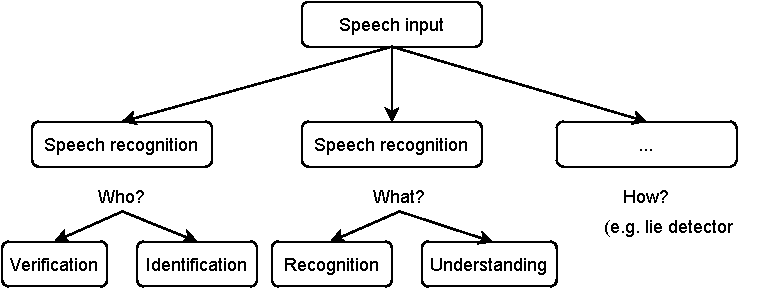
\includegraphics[width=0.8\textwidth]{speech-analysis}
	\caption{Speech input applications.}\label{fig:speech-input}
\end{figure}

In the speech input context, we need to ask three questions to obtain correct
answers: Who?, What?, and How?

\subsubsection*{Who?}
%Human speech has certain speaker-dependent characteristics, which means
%that speech input can serve to recognize a speaker. The computer is used to
%recognize an acoustic fingerprint of the speaker. 

Human speech has certain characteristics determined by a speaker. Hence,
speech analysis can serve to analyze \textit{who} is speaking, i.\ e.\ , to \textit{recognize a speaker} for his/her \textit{identification} and \textit{verification}. The computer identifies and verifies the speaker using an acoustic\footnote{An acoustic fingerprint is a digitally stored speech probe (e.\ g.\ , certain statement) of a person.} fingerprint.

\subsubsection*{What?}
%The central issue of speech input is to detect the speech contents themselves. A speech sequence is normally input to generate a piece of text. Typical applications are speech-controlled typewriters, language translation systems, or
%accessibility options for users with special needs.

Another main task of speech analysis is to analyze \textit{what has been said}, i.\ e.\ , to recognize and understand the speech signal itself. Based on speech sequence,
the corresponding text is generated.

\subsubsection*{How?}
Our third question relates to \textit{how a speech sample should be studied}. For example, a spoken sentence sounds differently if a person is angry or calm. One typical application is a lie detector.


\subsubsection{Speech Recognition}
In combination with speech synthesis, speech analysis enables us to implement media transformations.

The primary quality characteristic of each speech recognition session is determined by a probability of $ \leq 1 $ to recognize a word correctly. A word is always recognized only with a certain probability. Factors like environmental noise, room acoustics,
and the physical and psychical state of the speaker play an important role. 

For example, let's assume extremely bad individual word recognition with a probability of \(0.95\). This means that \(5\%\) of the words are incorrectly recognized. If we have a sentence with three words, the probability of recognizing the sentence correctly is
\(0.95 \times 0.95 \times 0.95 = 0.86\). 

This small example shows that a speech recognition system should have a very
high single-word recognition rate. Figure {\ref{fig:speech-recognition-principle}} shows the conceptual components of such a system.

%@@@@@@@@@@@@@@@@@@@@@@@@@@@@@@@@@@@@
%									@
%			FIGURE					@
%									@
%@@@@@@@@@@@@@@@@@@@@@@@@@@@@@@@@@@@@
\begin{figure}[hb!]
	\centering
	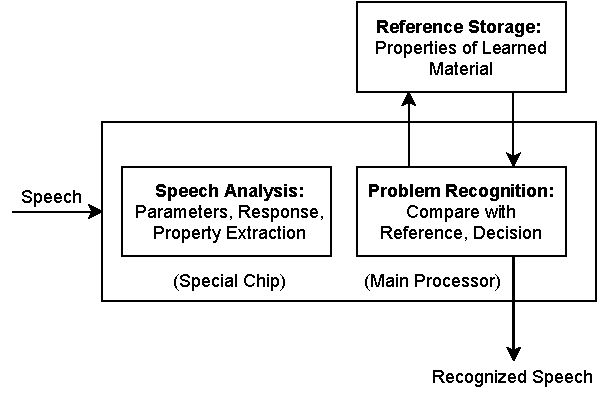
\includegraphics[width=0.8\textwidth]{speech-recognition-principle}
	\caption[The speech recognition principle]{The speech recognition principle: the tasks are distributed to system components by the basic principle ``extract characteristics to reduce data.''}\label{fig:speech-recognition-principle}
\end{figure}


The system is divided into system components according to a basic principle: ``Data Reduction Through Property Extraction''. 

 \textit{First}, speech analysis occurs where properties must be determined. Properties are extracted by comparison of individual speech element characteristics with a sequence of in advance given speech element characteristics. The characteristics are quantified where the concrete speech elements are present.


\textit{Second}, the speech elements are compared with existent references to determine the mapping to one of the existent speech elements. The identified speech can be stored,
transmitted or processed as a parameterized sequence of speech elements.

The principle shown in Figure {\ref{fig:speech-recognition-principle}} can be applied several times, each time referring to different characteristics. The application of the speech recognition principle can be divided into the steps shown in Figure {\ref{fig:speech-recognition-components}}.

%@@@@@@@@@@@@@@@@@@@@@@@@@@@@@@@@@@@@
%									@
%			FIGURE					@
%									@
%@@@@@@@@@@@@@@@@@@@@@@@@@@@@@@@@@@@@
\begin{figure}[ht!]
	\centering
		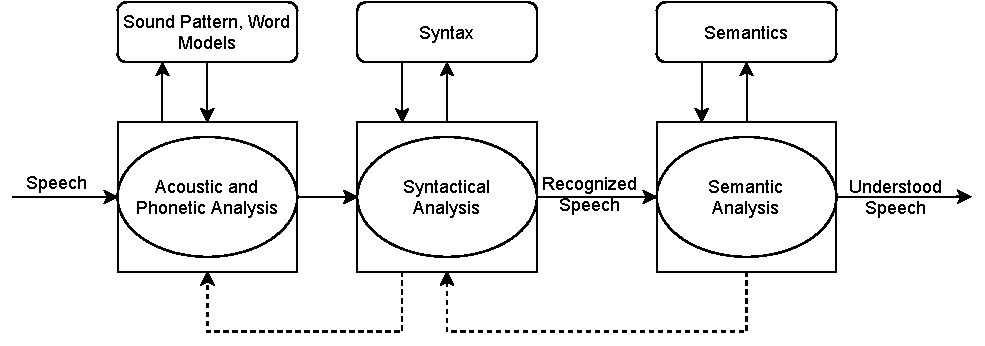
\includegraphics[width=\textwidth]{speech-recognition-components}
	\caption{Speech recognition components.}\label{fig:speech-recognition-components}
\end{figure}


The methods applied in the time and frequency ranges are:

\paragraph*{Acoustic and phonetic analysis}
In the first step, the principle is applied to a sound pattern and/or word model. An acoustical and phonetical \textit{analysis is performed}.

\paragraph*{Syntactic analysis}
The second step uses the speech units determined in the first step to run a syntactic analysis on them. This process can detect errors in the first run. It serves as an additional decision tool because the first step does not normally provide a final decision. The result is a \textit{recognized speech}.
	
\paragraph*{Semantic analysis}
The third step analyzes the semantics of the speech sequence recognized to this point. This step can detect errors from the previous decision process and remove them by using another interplay with other analytical methods. The implementation of this step is extremely difficult. The result of this step is an \textit{understood speech}.
	

\noindent These methods often work with characteristics in the time and/or frequency range. They are based on the same criteria and speech units (e.\ g.\ , formants or phonemes) as in speech output. 

\subsection[Transmission]{Speech Transmission}
Speech transmission is a field relating to highly efficient encoding of speech signals to enable low-rate data transmission, while minimizing noticeable quality losses. Some principles that are connected to speech generation and recognition are:

\subsubsection*{Pulse Code Modulation / Signal Form Coding}
Signal form encoding does not consider speech-dependent properties or parameters. Here, the goal is to achieve the most efficient coding of the audio signal. The data rate of a \gls{pcm}-coded stereo-audio signal with CD-quality requirements is:

\begin{align*}
rate & = 2 \times \frac{44,100}{s} \times \frac{16  {bits}}{8 bits/byte} \\
	& = 14,11,200 \times \frac{\cancel{bits}}{s} \times \frac{byte}{8\cancel{bits}}\\ 
	& = 14, 11, 200 \times \frac{byte}{8s}\\
	& = 1,76,400 \frac{byte}{s}\\
	& = 1,76,400 \times \frac{byte}{s} \times 8\: \textnormal{(\textnp{bits मा लैजान ८ ले गुणा गरेकाे})}  \\
	& = 14, 11, 200 bits/s\\
\end{align*}

%	\textnormal{\textnp{१}}
As a side note, telephone quality requires only $  64Kbit/s $ compared to $ 1,76,400byte/s $ for the case studied here. \gls{dpcm}
achieves $ 56Kbit/s $ in at least equal quality, while \gls{adpcm} enables a further reduction to $ 32Kbit/s $.

\subsubsection*{Source Encoding}
Parametric systems use source encoding. They utilize speech-specific characteristics to reduce data, for example the channel vocoder shown in Figure {\ref{fig:components-of-speech-transmission}}

%@@@@@@@@@@@@@@@@@@@@@@@@@@@@@@@@@@@@
%									@
%			FIGURE					@
%									@
%@@@@@@@@@@@@@@@@@@@@@@@@@@@@@@@@@@@@
\begin{figure}[ht!]
	\centering
		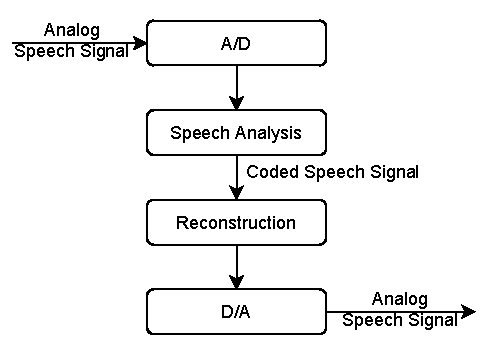
\includegraphics[width=0.6\textwidth]{components-of-speech-transmission}
	\caption[Components of a speech transmission system.]{Components of a speech transmission system using source encoding.}\label{fig:components-of-speech-transmission}
\end{figure}
%----------------------------figure end-----------------
A vocoder is an electronic mechanism that reduces speech signals to slowly varying signals that can be transmitted over communication systems of limited frequency bandwidth. A channel vocoder uses an enhanced subband encoding method.

In addition, the technique utilizes differences between \textit{voiced} and \textit{unvoiced} sounds. 
\begin{itemize}
	\item Unvoiced sounds are generated by means of a noise generator. 
	\item A pulse sequence is selected to generate voiced sounds.
\end{itemize}

\subsubsection*{Recognition/Synthesis Methods}

%Current research work attempts to further reduce the data volume by approximately $ 6Kbit/s $. The quality should always correspond to an uncompressed $ 64-Kbit/s $
%signal. Experts also study ways to reduce the transmission rate of speech signals by use
%of \textit{pure recognition-synthesis methods} (see Figure {\ref{fig:speech-recog-synthesis}}).

There have been attempts to reduce the transmission rate using pure recognition/synthesis methods. Speech analysis (recognition) follows on the sender side of a speech transmission system and speech synthesis (generation) follows on the receiver side (see Figure {\ref{fig:components-of-recognition-system}})

%@@@@@@@@@@@@@@@@@@@@@@@@@@@@@@@@@@@@
%									@
%			FIGURE					@
%									@
%@@@@@@@@@@@@@@@@@@@@@@@@@@@@@@@@@@@@
\begin{figure}[hb]
	\centering
		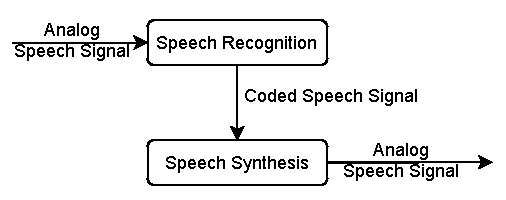
\includegraphics[width=0.8\textwidth]{components-of-recognition-system}
	\caption[Recognition/synthesis systems.]{Components of a recognition/synthesis system for speech transmission.}\label{fig:components-of-recognition-system}
\end{figure}


Only the speech element characteristics are transmitted, for example formants containing data about the center frequencies and bandwidths for use by digital filters.

\subsubsection*{Achievable Quality}
One of the most important aspects of speech and audio transmission in multimedia systems is the minimal achievable data rate in a defined quality. A data rate of less than $ 8Kbit/s $ for telephone quality can be achieved.

%@@@@@@@@@@@@@@@@@@@@@@@@@@@@@@@@@@@@
%									@
%			FIGURE					@
%									@
%@@@@@@@@@@@@@@@@@@@@@@@@@@@@@@@@@@@@
\begin{figure}[h]
	\centering
		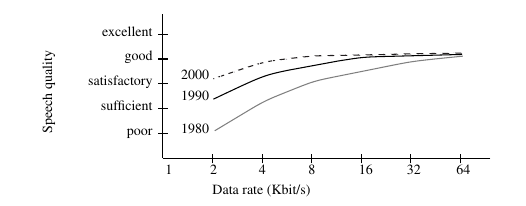
\includegraphics[width=\textwidth]{archievable-quality}
	\caption{Quality of compressed speech in relation to the compressed signal’s data rate.}\label{fig:archievable-quality}
\end{figure}


Figure \ref{fig:archievable-quality} relates the audio quality to the number of bits per sampling value. This ratio provides an excellent CD quality at a reduction of \(16 bits\) per sampling value to \(2 bits\) per sampling value, which means that only one eighth of the actual data rate is required to achieve this quality.
\newpage\thispagestyle{empty}
